% -----------------------------------------------
% Template for ICMC SMC 2014
% adapted and corrected from the template for SMC 2013,  which was adapted from that of  SMC 2012, which was adapted from that of SMC 2011
% -----------------------------------------------

\documentclass[twocolumn]{article}
\usepackage{icmcsmc2014}
\usepackage{times}
\usepackage{ifpdf}
\usepackage[english]{babel}
%\usepackage{cite}

%%%%%%%%%%%%%%%%%%%%%%%% Some useful packages %%%%%%%%%%%%%%%%%%%%%%%%%%%%%%%
%%%%%%%%%%%%%%%%%%%%%%%% See related documentation %%%%%%%%%%%%%%%%%%%%%%%%%%
%\usepackage{amsmath} % popular packages from Am. Math. Soc. Please use the 
%\usepackage{amssymb} % related math environments (split, subequation, cases,
%\usepackage{amsfonts}% multline, etc.)
%\usepackage{bm}      % Bold Math package, defines the command \bf{}
%\usepackage{paralist}% extended list environments
%%subfig.sty is the modern replacement for subfigure.sty. However, subfig.sty 
%%requires and automatically loads caption.sty which overrides class handling 
%%of captions. To prevent this problem, preload caption.sty with caption=false 
%\usepackage[caption=false]{caption}
%\usepackage[font=footnotesize]{subfig}


%user defined variables
\def\papertitle{Detecting the Awesome Guitar Solo Moment with GuitarFace}
\def\firstauthor{Regina Collecchia}
\def\secondauthor{Roshan Vidyashankar}
% \def\thirdauthor{Third author}

% adds the automatic
% Saves a lot of ouptut space in PDF... after conversion with the distiller
% Delete if you cannot get PS fonts working on your system.

% pdf-tex settings: detect automatically if run by latex or pdflatex
\newif\ifpdf
\ifx\pdfoutput\relax
\else
   \ifcase\pdfoutput
      \pdffalse
   \else
      \pdftrue
\fi

\ifpdf % compiling with pdflatex
  \usepackage[pdftex,
    pdftitle={\papertitle},
    pdfauthor={\firstauthor, \secondauthor},
    bookmarksnumbered, % use section numbers with bookmarks
    pdfstartview=XYZ % start with zoom=100% instead of full screen; 
                     % especially useful if working with a big screen :-)
   ]{hyperref}
  %\pdfcompresslevel=9

  \usepackage[pdftex]{graphicx}
  % declare the path(s) where your graphic files are and their extensions so 
  %you won't have to specify these with every instance of \includegraphics
  \graphicspath{{./figures/}}
  \DeclareGraphicsExtensions{.pdf,.jpeg,.png}

  \usepackage[figure,table]{hypcap}

\else % compiling with latex
  \usepackage[dvips,
    bookmarksnumbered, % use section numbers with bookmarks
    pdfstartview=XYZ % start with zoom=100% instead of full screen
  ]{hyperref}  % hyperrefs are active in the pdf file after conversion

  \usepackage[dvips]{epsfig,graphicx}
  % declare the path(s) where your graphic files are and their extensions so 
  %you won't have to specify these with every instance of \includegraphics
  \graphicspath{{./images/}}
  \DeclareGraphicsExtensions{.eps}

  \usepackage[figure,table]{hypcap}
\fi

%setup the hyperref package - make the links black without a surrounding frame
\hypersetup{
    colorlinks,%
    citecolor=black,%
    filecolor=black,%
    linkcolor=black,%
    urlcolor=black
}


% Title.
% ------
\title{\papertitle}

 \twoauthors
   {\firstauthor} {Stanford University \\ %
     {\tt \href{mailto:colleccr@ccrma.stanford.edu}{colleccr@ccrma.stanford.edu}}}
   {\secondauthor} {Stanford University \\ %
     {\tt \href{mailto:rvid@ccrma.stanford.edu}{rvid@ccrma.stanford.edu}}}
%   {\thirdauthor} { Affiliation3 \\ %
%     {\tt \href{mailto:author3@smcnetwork.org}{author3@smcnetwork.org}}}


% ***************************************** the document starts here ***************
\begin{document}
%
\capstartfalse
\maketitle
\capstarttrue
% headline image of 10 guitar faces
% \capstartfalse
% \twocolumn[\begin{@twocolumnfalse}
% \begin{tabular}
%\begin{minipage}{17.2cm} 
%\begin{center} \begin{tabular}{ccccc p{17.2cm}}
%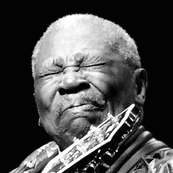
\includegraphics[width=0.18\linewidth]{images/goodgf/gf015.png} &
%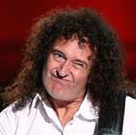
\includegraphics[width=0.18\linewidth]{images/goodgf/gf025.png} &
%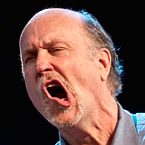
\includegraphics[width=0.18\linewidth]{images/goodgf/gf033.png} &
%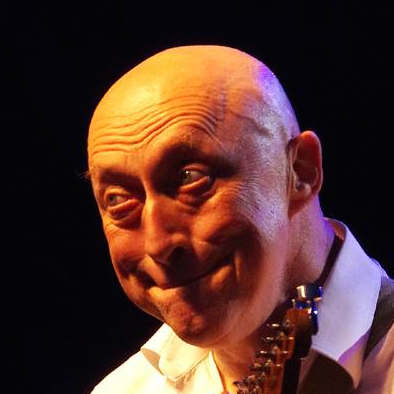
\includegraphics[width=0.18\linewidth]{images/goodgf/gf036.png}&
%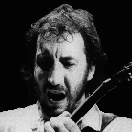
\includegraphics[width=0.18\linewidth]{images/goodgf/gf066.png} \\
%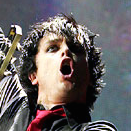
\includegraphics[width=0.18\linewidth]{images/goodgf/gf067.png} &
%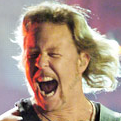
\includegraphics[width=0.18\linewidth]{images/goodgf/gf071.png} &
%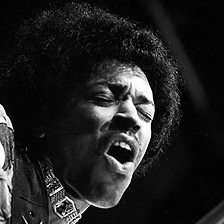
\includegraphics[width=0.18\linewidth]{images/goodgf/gf075.png} &
%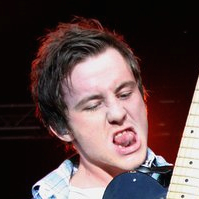
\includegraphics[width=0.18\linewidth]{images/goodgf/gf090.png} &
%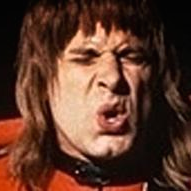
\includegraphics[width=0.18\linewidth]{images/goodgf/gf105.png} 
%\end{tabular} \end{center}
%\end{minipage}
% \capstarttrue
% \end{@twocolumnfalse}]
%
\begin{abstract}
It is difficult to tackle the problem of identifying ``awesomeness" without facing serious judgment calls on musical taste. One thing that does give away the joy and energy contained in a moment is the facial expression of a performer. Aiming to recognize the face a musician makes during an awesome musical moment, we created \textit{GuitarFace}, a Mac application with facial recognition via the OpenCV library. The user is a musician practicing their instrument either alone or across the network with a friend. Gameplay is a mix of MIDI guitar input visualization, counts of musical events like big jumps in pitch or power chords, and events initiated by making a guitar face. In another sense, GuitarFace is the beginnings of a ``funny face" detector.
\end{abstract}
%

\section{Introduction}\label{sec:introduction}
Before we went the route of facial detection, we were interested in detecting moments of high quality and expressiveness in guitar solos. However, we soon realized that even if we had a perfect feature set that everyone agreed upon as the common ingredients in all great guitar solos, problems like pitch detection, source separation, and extra-musical features like live performance posed serious obstacles. Thus, we narrowed our goals to focus only on the extra-musical events: the way a guitarist stands and holds his or her guitar, the way they move around stage and engage with fans and fellow bandmates, and of course, the face they make during all of this. 

Software like Guitar Hero succeeds in delivering some of the emotion of being on stage to the living room, and may even increase the musicianship of players. In the same vein, GuitarFace is meant to give users that feeling as they practice their instrument. Otherwise, we were motivated by humor, joy, and the ``laptop musician problem," referring to how the performer-computer interaction tends to alienate an audience during a live show. We could see facial recognition technology to aide live performance production, by cueing new camera views or triggering graphical events such as virtual fire projected behind the performer. It could also be used for something more musical, like turning on a guitar effect preset to double octaves. With that said, we have not totally resolved how a camera could track a performer's face unobtrusively were they to use it on stage; this research is instead directed at the detection of guitar face.

\subsection{Background}
Facial recognition is a rapidly advancing field of machine learning and computer vision, now built in to popular services like Facebook and applications like iPhoto. Many models for facial recognition use support vector machines (SVM), active appearance models (AAM), Haar classifiers, and other supervised learning models

\section{Method}
After reviewing hundreds of photos found by an image search for ``guitar face," we named 7 facial features that we believed to be more guitar face than not:
\begin{enumerate}
\item mouth open, as if in pain
\item mouth tightly pursed, slightly smiling
\item eyes (pinched) closed
\item lips unaligned, mouth open
\item tongue out
\item head tilted back or to the side
\item mouth in an `O' shape, as if yelling
\end{enumerate}
Working with the time constraints and resources that we had, we designed algorithms for filtering the state of the mouth and the eyes, and triggered a ``guitar face event" whenever the eyes were closed or the mouth was open, past a threshold of 0.18 times the height of the face.\footnote{Here ``face" refers to the 66-point matrix drawn by [citation], so the height of the ``face" would be from the bottom of the chin to the top of the left eyebrow. See Figure X.}

\section{Implementation}
Our attempts to detect and track guitar face were in 3 stages:
\begin{itemize}
\item using the built-in face tracker in OpenCV based on Haar-like features;
\item using a model for face-tracking developed by Jason Saragih and ported to C++ by Kyle McDonald, annotating the face with 66 coordinates; and
\item exploring SVM and AAM based trainers.
\end{itemize}
We had mixed success with all of these approaches, discussed more in Section 4. 

We first used the built-in face tracker in OpenCV, which draws a rectangle around the face with pretty strong accuracy. We did not find the other (Haar-based) facial feature trackers to be accurate enough or work well enough in real-time. We used Kyle McDonald's C++ version of Jason Saragih's code for face-tracking, which annotates the face with 66 coordinates. It works best on faces that are straight on because of the symmetry component in the face-tracking algorithm, so we had difficulty when applying it to tilted faces. Finally, we attempted to manually train an active appearance model by annotating 20 photographs by hand, using Radhika Vathsan's trainer. 



Using the built in face detector in OpenCV, the rectangular area around the face was detected with high accuracy and only a few lines of code. The strongest feature that we assimilated to ``guitar face" was an open mouth, so we tackled this feature first. We tried a few different techniques to detect this feature with interesting results and mixed success.

 We assumed that the face was straight on. 

\section{Evaluation}\label{sec:eval}
Into the GuitarFace application, we built in a key press to allow us to say that we were making a guitar face, and recorded how many times our software successfully identified the face. For the black pixel method, we had a X success rate. For tracking the height of the eyes and lips, guitar faces were detected X\% of the time. 

\section{Conclusion and Future Work}\label{conclusion}

%\subsection{Equations}
%Equations should be placed on separated lines and numbered.
%The number should be on the right side, in parentheses.
%\begin{equation}
%E=mc^{2}.
%\label{eq:Emc2}
%\end{equation}


%%%%%%%%%%%%%%%%%%%%%%%%%%%%%%%%%%%%%%%%%%%%%%%%%%%%%%%%%%%%%%%%%%%%%%%%%%%%%
%bibliography here
% \bibliography{guitarface}
% http://opencv.org
\end{document}
